% !TeX program = lualatex
\documentclass[../skript/main.tex]{subfiles}
\usepackage{tikz}
\usetikzlibrary{arrows.meta,calc,positioning}
\graphicspath{{\subfix{../figures/}}}
\begin{document}

\chapter{Die Zweierkomplementdarstellung-test}
\label{chap:zweierkomplement}

Die Zweierkomplementdarstellung (2K) kodiert ganze Zahlen so, dass Addition und Subtraktion
als Modulo-\(2^n\)-Arithmetik mit denselben Schaltungen wie bei vorzeichenlosen Werten funktionieren.

\section{Wertebereich und Interpretation}
Für \(n\)~Bit gilt: \(\min=-2^{n-1}\), \(\max=2^{n-1}-1\).
Das höchstwertige Bit hat das negative Gewicht \(-2^{n-1}\).

\section{Zahlenstrahl (8 Bit)}
\begin{figure}[H]\centering
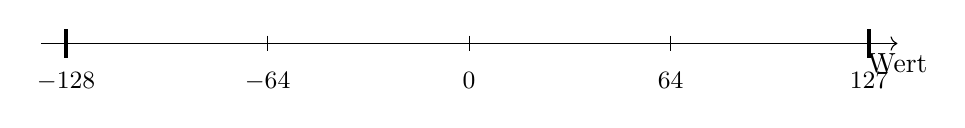
\begin{tikzpicture}[x=0.04cm,y=1cm]
  \draw[->] (-136,0) -- (136,0) node[below] {Wert};
  \foreach \x/\lab in {-128/{$-128$}, -64/{$-64$}, 0/{$0$}, 64/{$64$}, 127/{$127$}}{
    \draw (\x,0.1) -- (\x,-0.1) node[below=4pt] {\small \lab};
  }
  \draw[very thick] (-128,0.18)--(-128,-0.18);
  \draw[very thick] (127,0.18)--(127,-0.18);
\end{tikzpicture}
\caption{8-Bit-Zweierkomplement auf dem Zahlenstrahl.}
\end{figure}

\end{document}
